%Experimental Results and Analysis – in this section you should show the quantitative results – charts and tables. Analyze the results by explaining and highlighting what is important on them in terms of your goals and what is bad. You should explain the strange results too.

\section{Results and Analysis of Two learning rate model} %TODO better section name 
\label{sec:results} 

In this section we present and analyse our most important result, i.e. the \emph{Two learning rate} model \ref{sec:our-two-lambdas}. Other results are shortly discussed in the appendix \ref{sec:appendix-results}. We start by comparing it to previous models \ref{sec:results-comparison}

%V ďalšej časti prezentujte vlastný prínos a vlastné výsledky porovnajte s výsledkami iných. Charakterizujte použité metódy.
%Vyhýbajte sa používaniu žargónu.
%Používajte starú múdrosť: 1 obrázok je viac než 1000 slov.

\section{Analysis of the Two learning rate model} 
\label{sec:analysis}
\label{sec:results} 

In this section we present in--depth analysis of the Two learning rate model.  
TODO Explain how it was measured (runs, epochs, stopping) \\
TODO Explain / Make up hypotheses why it behaves as measured (Future work). \\

%Experimental Results and Analysis – in this section, you should show the quantitative results – charts and tables. Analyze the results by explaining and highlighting what is important on them in terms of your goals and what is bad. You should explain the strange results too.

%V ďalšej časti prezentujte vlastný prínos a vlastné výsledky porovnajte s výsledkami iných. Charakterizujte použité metódy.
%Vyhýbajte sa používaniu žargónu.
%Používajte starú múdrosť: 1 obrázok je viac než 1000 slov.

\subsection{4-2-4 Encoder} 
\label{sec:results-auto4} 

%==================================================================
\paragraph{Introduction.} 
\label{sec:results-auto4-introduction} 
In this section, we analyse performance of TLR for a broad range of parameters $\lambda_h$ and $\lambda_v$. The network architecture is only 4-2-4~
(\ref{sec:datasets-auto4}) what allows us to run plethora of simulations. There were two kinds of simulations. First are \emph{two dimensional maps (TDM)}, where $\lambda_v$ is plotted on the $x$ axis, $\lambda_h$ on the $y$ axis and color is used for the $z$ axis. Second are \emph{timelines}  on which success per epoch was plotted for best configuration found by TDM. For creating TDM we ran 500 networks for each pair ($\lambda_v$, $\lambda_h$) and for timelines we ran 10000 networks. After the simulations ended, the average for each configuration was plotted. The networks were trained while $patSucc^F \neq 1$ or $epoch < Epoch_{\rm max}$ where $Epoch_{\rm max}$ was set to 100,000 in TDM and 1,000,000 in timelines. Note that most of the plots are in \emph{logarithmic} scale. 

%============================================================

\subsubsection{Comparison} 
\label{sec:tlr-auto4-cmp} 

In the following table~(\ref{tab:results-cmp-auto4}) we can see the comparison of the most important models which we analysed on the \emph{4-2-4 encoder} task. We achieved an improvement of BAL $patSucc^F$ from $62.7\%$ to $93.1\%$ by using two different learning rates~(\ref{sec:our-tlr}). This result was improved further to $99.86\%$ by preselecting networks based on initial weights~(\ref{sec:sim-exp-candidates}). This proved that hidden distance and representation convexity are important attributes of BAL~(\ref{sec:results-candidates}). 

On the other hand, many of the analysed models achieved poorly. Notably we tried modified GeneRec learning rules~(\ref{sec:models-generec-modifications}) on BAL, calling this model \emph{BAL GeneRec Learning Rules (BAL GLR)}. This led to no good results. Also, \emph{BAL-recirc}~(\ref{sec:our-bal-recirc}) achieved worse than BAL. We experimented with \emph{momentum} in section~(\ref{sec:results-momentum}), symmetric version of BAL in section~(\ref{sec:our-bal-sym}) and other modification but all without significant improvement in success. 

\begin{table}[H] 
  \centering
    \begin{tabular}{|l|l|l|l|l|}
    \hline
    Algorithm (section)&$\lambda_h$&$\lambda_v$&$patSucc^F$ &Epochs\\ %&SEM(success) \\
    \hline
    BP~(\ref{sec:models-bp}) &2.4 &2.4 &100&60\\ %&5.1\\
    \hline
    GR~(\ref{sec:models-generec}) &0.6 &0.6 &90&418\\ %&28\\
    \hline
    GR Sym~(\ref{eq:models-generec-learning-rule-sym}) &1.4 &1.4 &56&88\\ %&2.9\\
    \hline
    GR Mid~(\ref{eq:models-generec-learning-rule-mid}) &2.4 &2.4 &92&60\\ %&3.4\\
    \hline
    CHL~(\ref{sec:models-chl}) &1.2 &1.2 &56&77\\ %&1.8\\
    \hline
    BAL~(\ref{sec:models-bal})&0.9 &0.9 &62.7& 5136.11\\ %&2.0e+08\\
    \hline
    BAL TLR~(\ref{sec:our-tlr})&0.0002  & 500&93.12&5845.01\\ %&1.52e+08\\
    \hline
    BAL TLR Can~(\ref{sec:sim-exp-candidates})&0.0002&500&99.86&150.417\\ %&5,070,000\\
    \hline
    BAL Recirc~(\ref{sec:our-bal-recirc})&0.0001&1.0&36.0&1221.6\\ %&4.31e+07\\
    \hline
    BAL GLR~(\ref{sec:models-generec-modifications})& any & 0 & 0 & N/A \\ 
    \hline 
    %TODO Symmetric BAL 
    \end{tabular}
  \caption{Comparing performance of different models on the \emph{4-2-4 encoder} task. Data for BP, GR, GR Sym, Gr Mid and CHL are taken from~\citet{o1996bio}.} 
  \label{tab:results-cmp-auto4}
\end{table}

Note that when comparing runtime in table~\ref{tab:results-cmp-auto4} based on \emph{epochs} we must be aware of that GeneRec and BAL-recirc epochs take longer than others. That is because the recirculation step~(\ref{sec:models-generec-activation}) where usually about 5--15 iterations are necessary for activation to settle~(\ref{sec:generec-fluctuation}). Thus the 418 epochs of GeneRec are comparable to the 5845 epochs of TLR in terms of compuration time. 
 

%============================================================
\subsubsection{Two learning rates} 
\label{sec:tlr-auto4}

In figure~\ref{fig:results-tlr-auto4-performance} we compare success rate for range of $\lambda_v$ and $\lambda_h$. It~is interesting that the subspace with best achieving networks is around the half line $[(10, 0.001),\,(10^9, 0.001)]$. That means the performance mainly depends on $\lambda_h$ while a constraint on $\lambda_v$ is added. See the plot for epochs, where a \emph{ridge} occurred around line $[(0.01, 0.0002),\,(10^9, 0.0002)]$. Unfortunatelly, we can only guess what is the reason behind this ridge. Maybe it~is related to $Epoch_{\rm max}$ and the fact that we are calculating epochs only from successful networks. Therefore, successful networks having $\lambda_h > 10^{-6}$ need to converge using $\lambda_v$, because otherwise they would fail to converge because of $\lambda_h \cdot Epoch_{\rm max} < 1$. 

Note that the success space is robust and therefore it is possible to find it by stochastic methods such as Monte Carlo. This approach is needed as finding the optimal values of $\lambda_v$ and $\lambda_h$ could take long using the trivial exhaustive search. 

%======== (3D) L1 x L2 x epochs =========
%======== (3D) L1 x L2 x patSuccF =========
\begin{figure}[H]
  \centering
  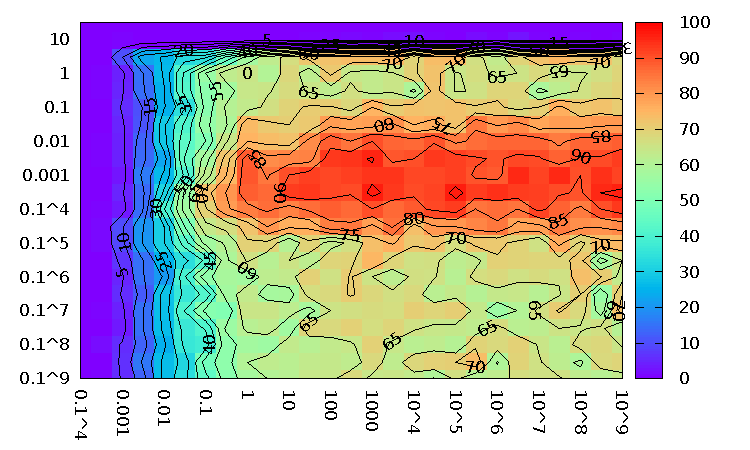
\includegraphics[width=0.49\textwidth]{img/tlr-auto4-success.pdf}   
  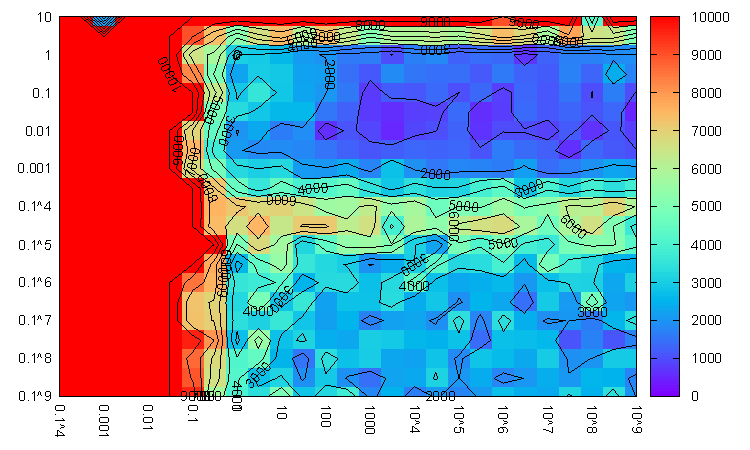
\includegraphics[width=0.49\textwidth]{img/tlr-auto4-epoch.pdf}     
  \caption{TLR success and epochs needed for successful networks on the \emph{4-2-4 encoder} task with $\sigma = 2.3$ and $\mu = 0.0$ best being $96.5\$$ with $\lambda_h=0.0003$ and $\lambda_v=1000.0$.}
  \label{fig:results-tlr-auto4-performance}
\end{figure}

Note the inconsistency between table~\ref{tab:results-cmp-auto4}, where 93.12\% success was stated for TLR, and in figure~\ref{fig:results-tlr-auto4-performance} where it was 96.5\%. This is explained by the \emph{law of big numbers}. In the first case the average performance of 10000 networks were used, thus the result is likely to mirror the reality. In the second case only 200 networks were used for a particular $(\lambda_v,\,\lambda_h)$ pair. As there were about 50 candidates for best achievers, it was likely that some of them will achieve better than in the long run. 

In figure~\ref{fig:results-tlr-auto4-epoch} the success timeline for TLR with best $\lambda_h$ and $\lambda_v$ is analysed. We see that the success rate increases even after $10^5$ epochs and our intuition tells us that it will continue even after $10^6$ epochs. Another observation is that $patSucc^B$ first follows $patSucc^F$ for about 100 epochs, but then it stagnates at rate $\approx0.8$. We find this hard to explain as both the architecture and data are symmetric. 

%======== (2D) best TLR on ALL_SUCC x epoch (std-dev) ==========
\begin{figure}[h]
  \centering
  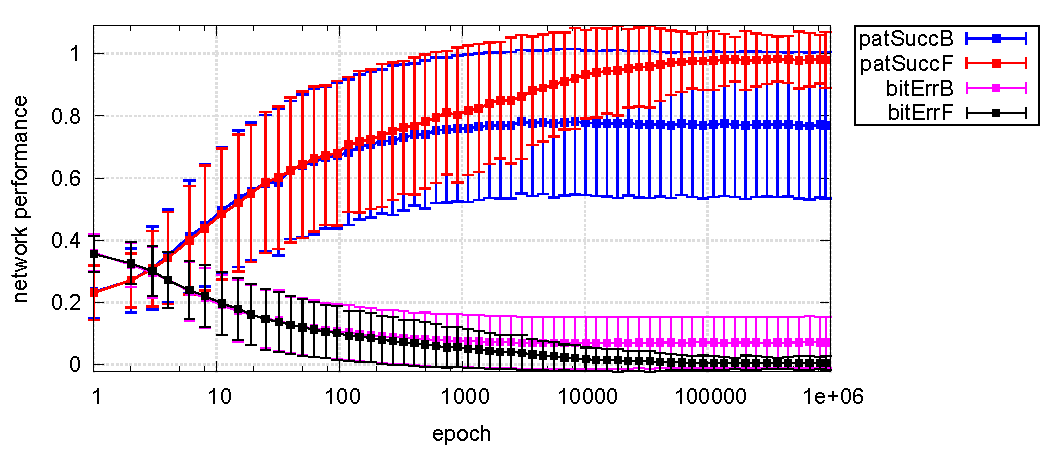
\includegraphics[width=0.8\textwidth]{img/tlr-auto4-best-perf.pdf}\\
  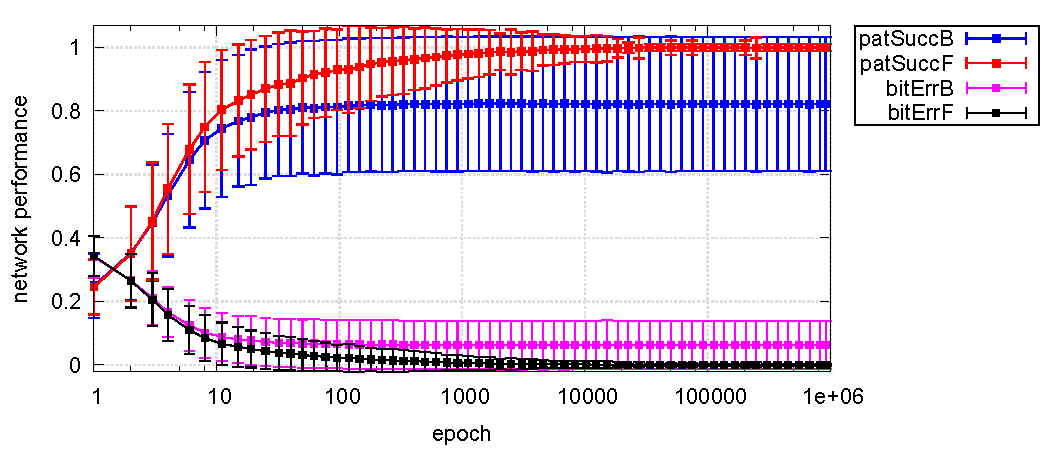
\includegraphics[width=0.8\textwidth]{img/tlr-auto4-best-can.pdf}      
  \caption{TLR success timeline for the \emph{4-2-4 encoder} task with $\lambda_h=0.0002$ and $\lambda_v=500$. Top plot without candidate selection and bottom plot with candidates selection.}
  \label{fig:results-tlr-auto4-epoch} 
\end{figure}

%============================================================
\subsubsection{Hidden activations} 
\label{sec:tlr-auto4-hidden}

In figures~\ref{fig:results-hidden-activations-bal} and~\ref{fig:results-hidden-activations-tlr} we show forward hidden activations. Each color represents the forward hidden representation of one of the four inputs in the \emph{4-2-4 encoder} task. As the hidden layer size is 2 the hidden activation could be mapped to two dimensional space. The plotted activations start at $epoch=0$ depicted with black squares and continue as outlined by the the lines. 

The main difference between TLR and BAL seems to be the speed of activation change. For BAL, as shown in figure~\ref{fig:results-hidden-activations-bal}, we have a step of size 0.6, which corresponds to four, one for each input, weight updates. Another observation is that after some initial steps BAL tends to stop the activation change. This could be contributed to settling $|H^F-H^B| \approx 0$ as discussed in~(\ref{sec:our-hidden-activation}). 

Another source of error could be \emph{non--convex} hidden activation initializations. In the beginning the weight matrices are initialized by random what leads to random hidden activations. And if the hidden activations are also non--convex in the end then it~is impossible to perfectly classify on the hidden--to--visible layer due the linear separability theorem discussed in section~(\ref{sec:models-perceptron}). Therefore if the network had non--convex hidden activations in the beginning, then it must \emph{escape} the non--convex state and this could introduce problems. 

%===== hidden activation timelines with commentaries (for TLR, BAL, GeneRec) 
% 2x success, 2x error (wrong settle, divergence) 

\begin{figure}[H]
  \centering
  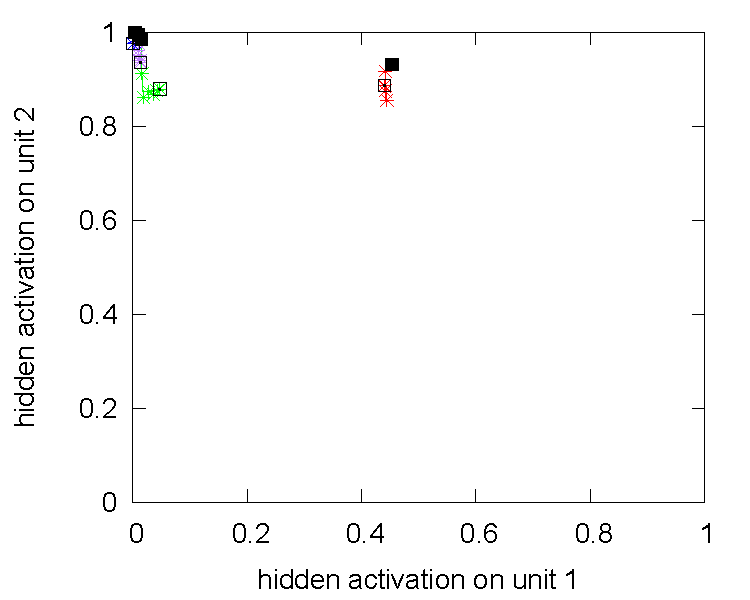
\includegraphics[width=0.45\textwidth]{img/hid-bal-bad-init.pdf}  
  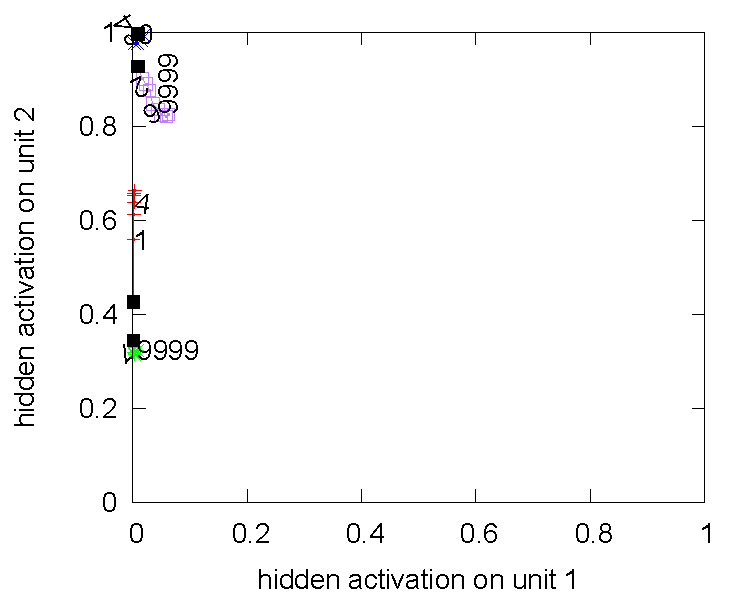
\includegraphics[width=0.45\textwidth]{img/hid-bal-bad-convex.pdf}  \\
  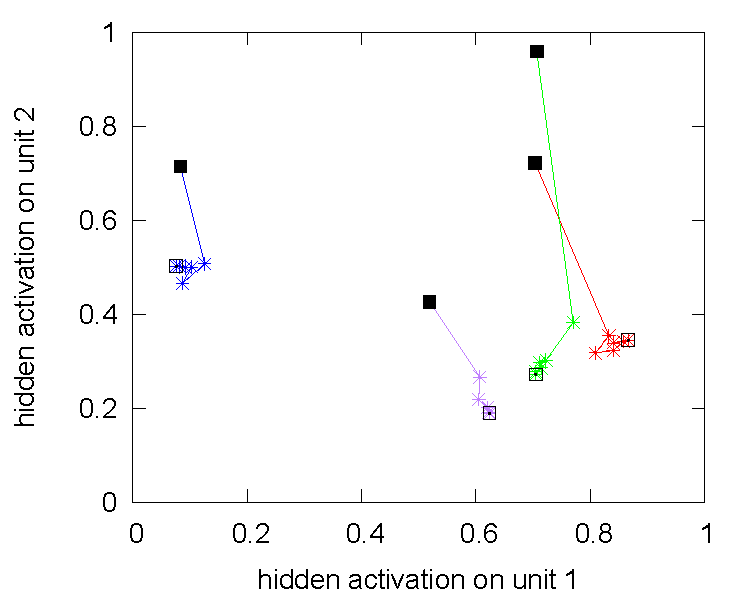
\includegraphics[width=0.45\textwidth]{img/hid-bal-bad-step.pdf}  
  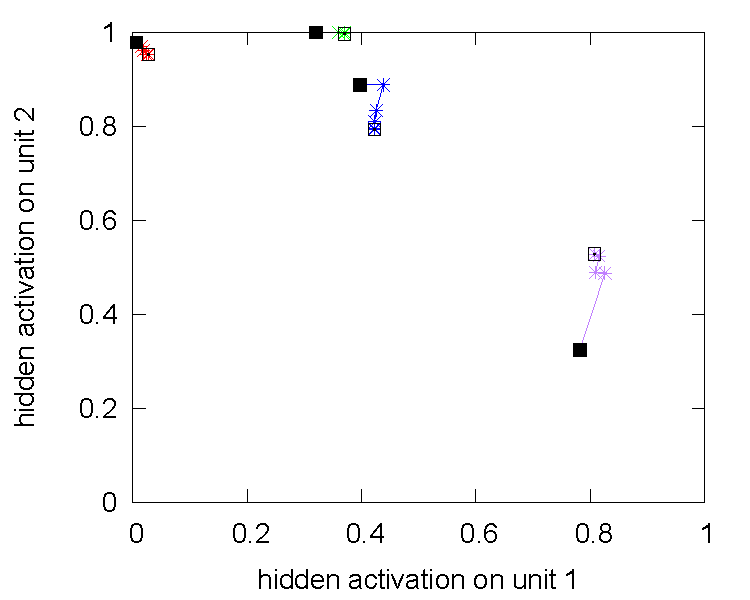
\includegraphics[width=0.45\textwidth]{img/hid-bal-bad-stagnation.pdf}  \\
  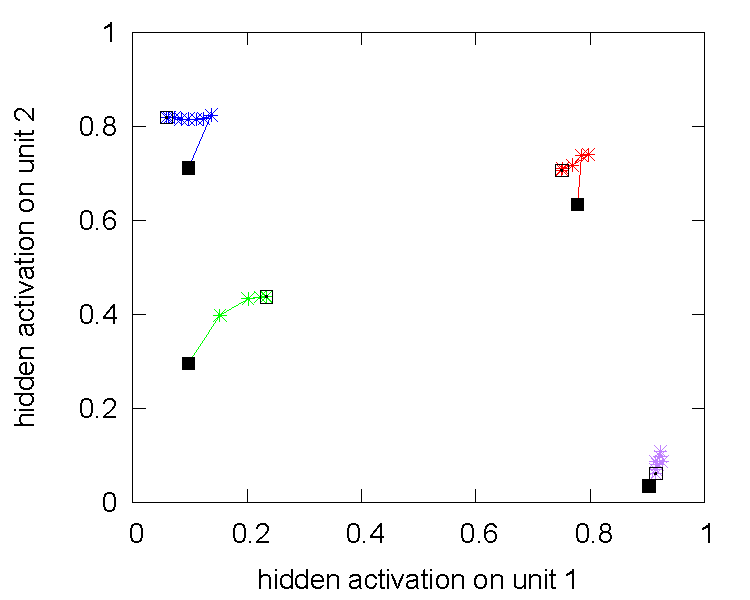
\includegraphics[width=0.45\textwidth]{img/hid-bal-good-init.pdf}  
  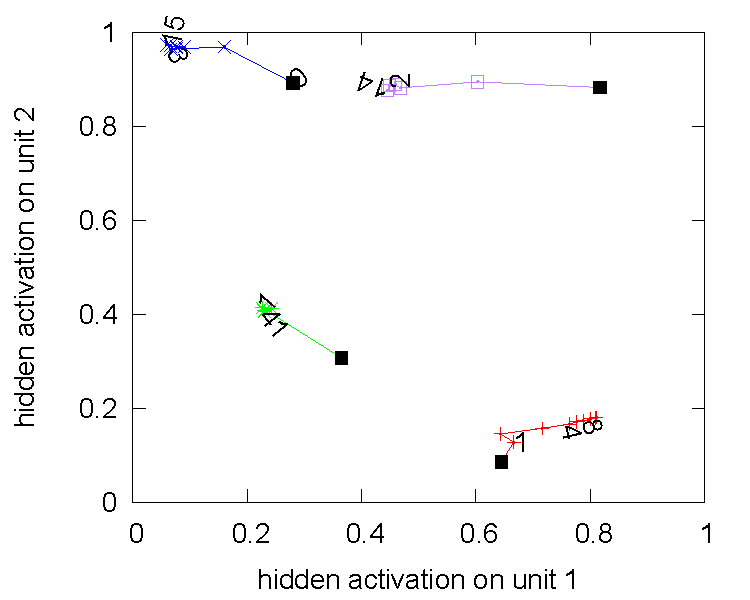
\includegraphics[width=0.45\textwidth]{img/hid-bal-good-convex.pdf}  \\
  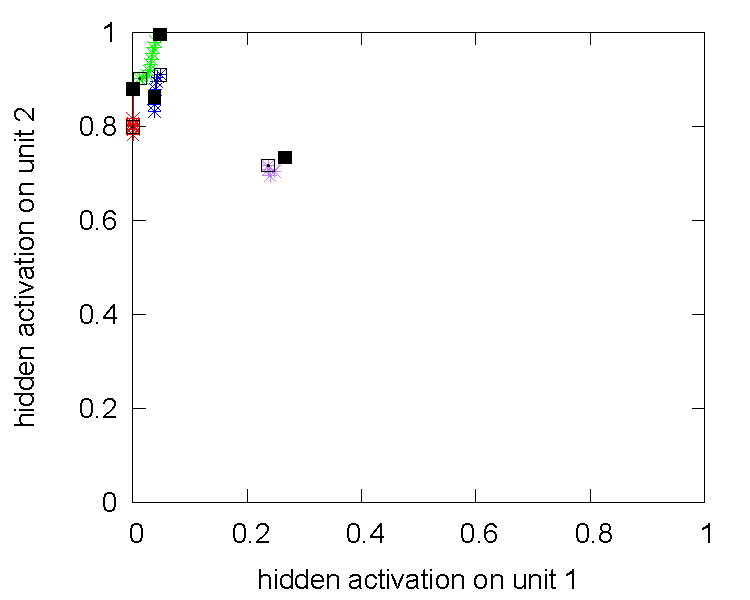
\includegraphics[width=0.45\textwidth]{img/hid-bal-good-step.pdf}  
  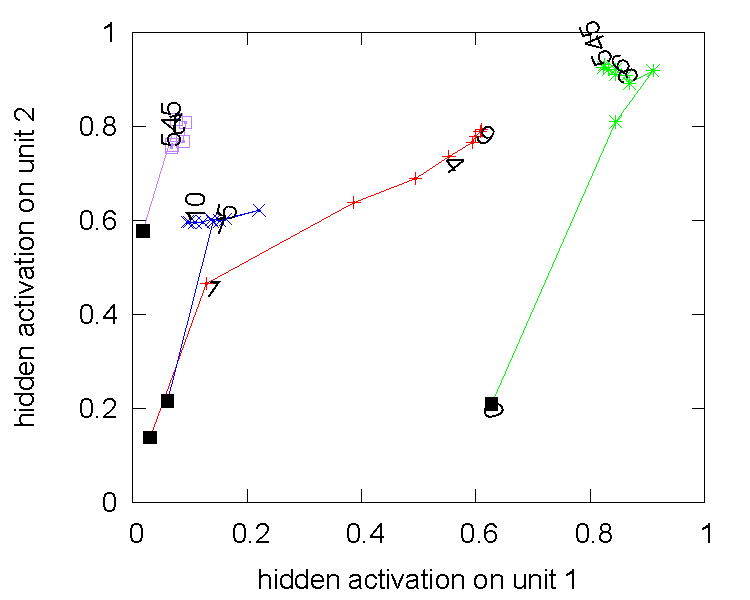
\includegraphics[width=0.45\textwidth]{img/hid-bal-good-stagnation.pdf}  \\ 
  \caption{\emph{BAL} hidden activations on the \emph{4-2-4 encoder}. Top $2\times2$ are {\bf un}successful networks and bottom $2\times2$ successful ones. There were about 100 epochs with change in activation.}
  \label{fig:results-hidden-activations-bal}
\end{figure}

\begin{figure}[H]
  \centering
  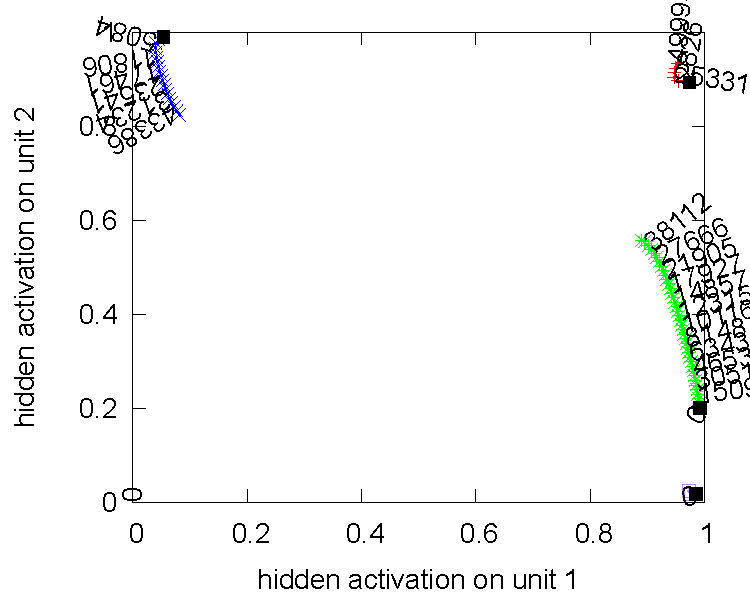
\includegraphics[width=0.45\textwidth]{img/hid-tlr-bad-static.pdf}  
  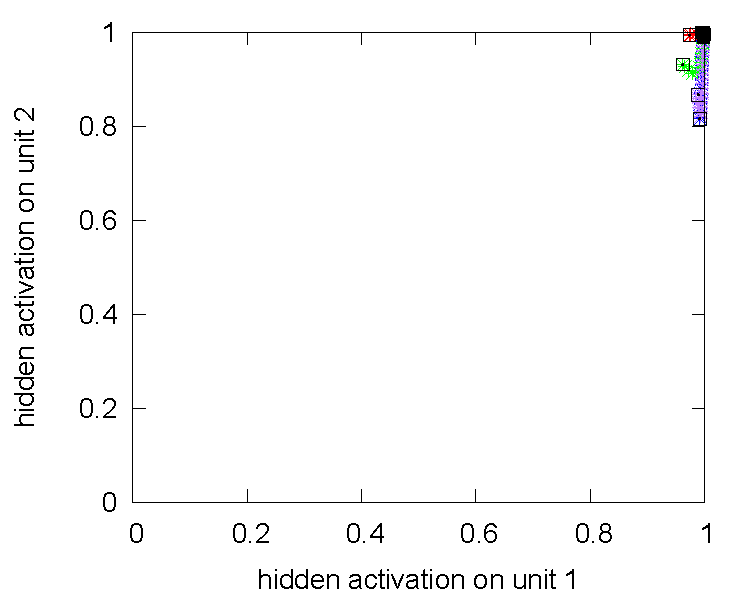
\includegraphics[width=0.45\textwidth]{img/hid-tlr-bad-tiny.pdf}  
  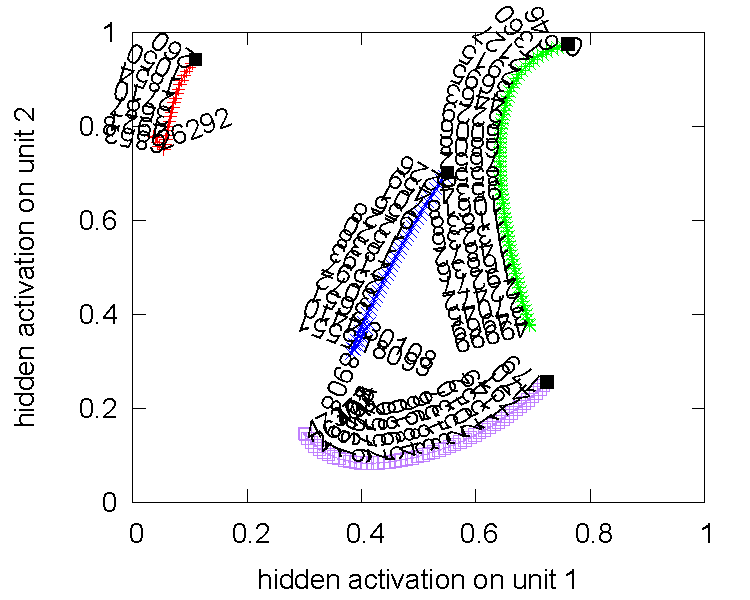
\includegraphics[width=0.45\textwidth]{img/hid-tlr-bad-init.pdf}  
  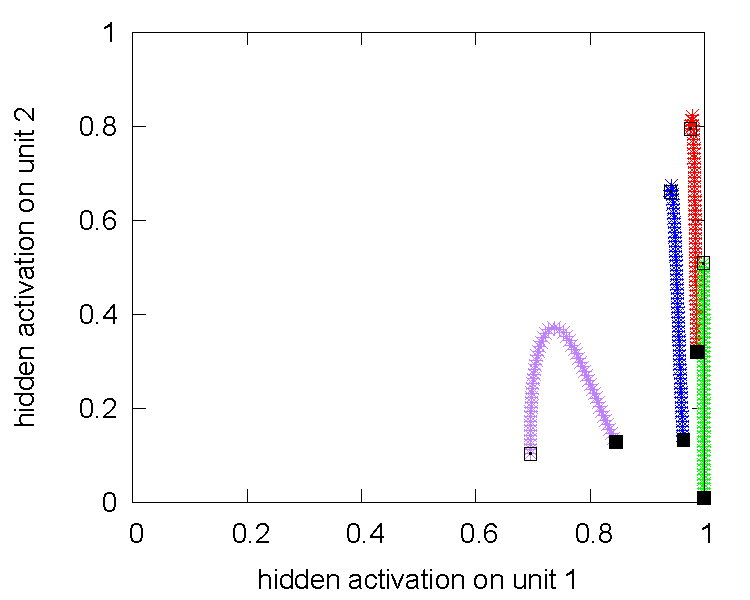
\includegraphics[width=0.45\textwidth]{img/hid-tlr-bad-weird.pdf}  
  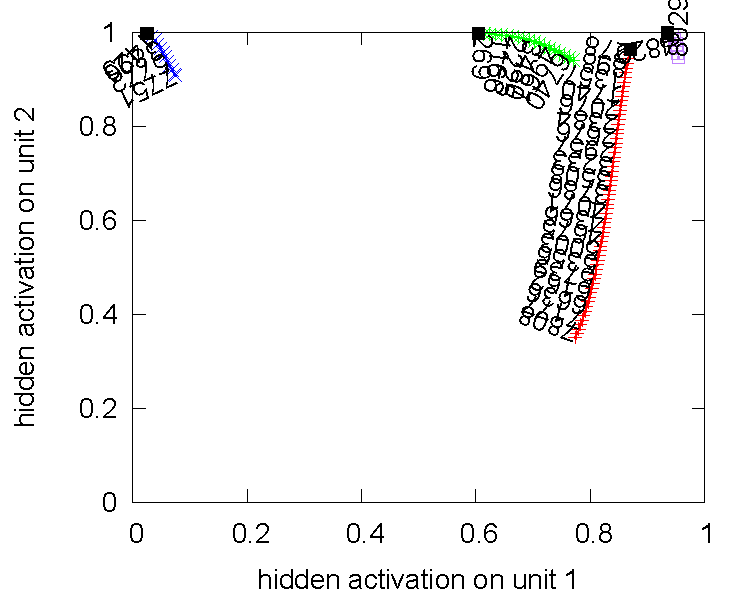
\includegraphics[width=0.45\textwidth]{img/hid-tlr-good-static.pdf}  
  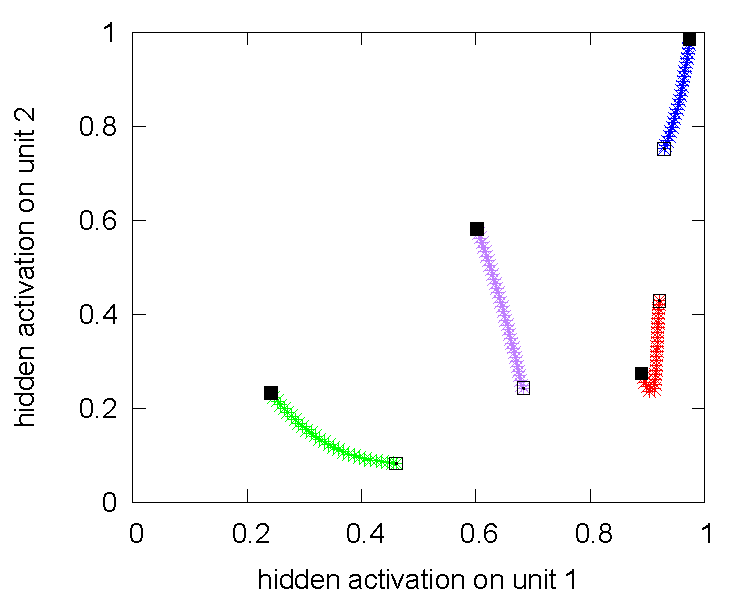
\includegraphics[width=0.45\textwidth]{img/hid-tlr-good-tiny.pdf}  
  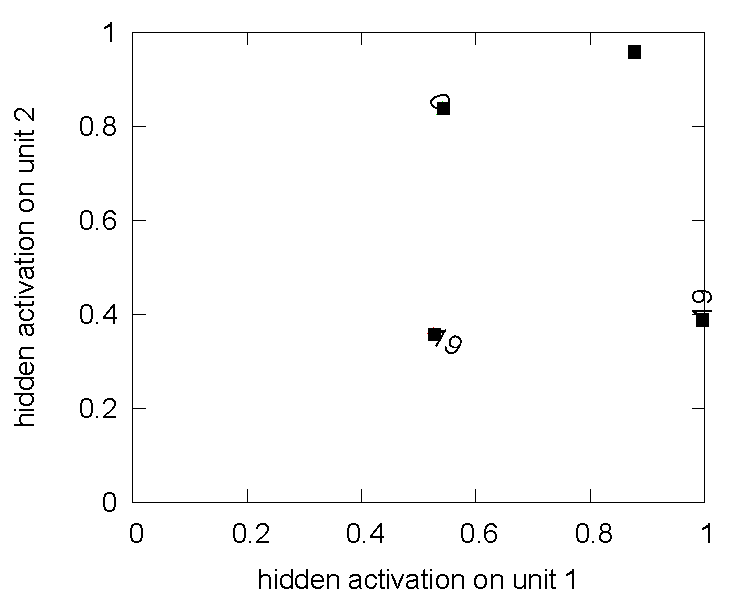
\includegraphics[width=0.45\textwidth]{img/hid-tlr-good-init.pdf}  
  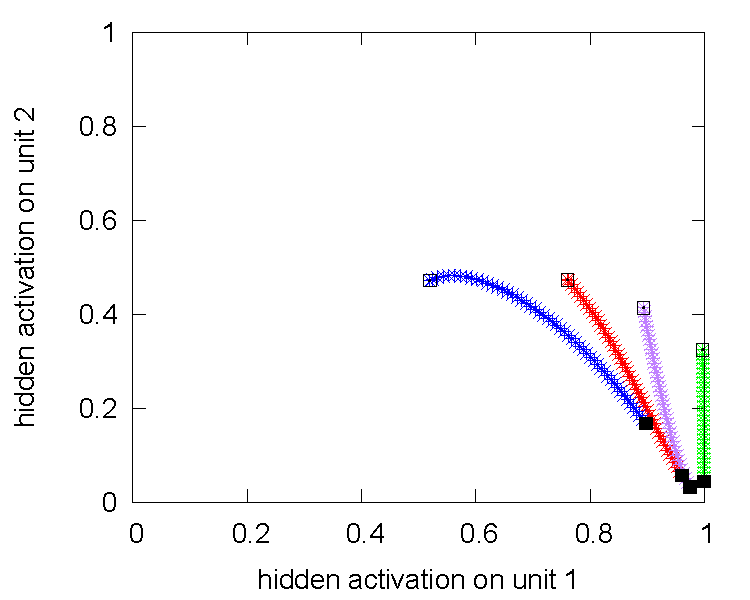
\includegraphics[width=0.45\textwidth]{img/hid-tlr-good-weird.pdf}  
  \caption{\emph{TLR} hidden activations on the \emph{4-2-4 encoder}. Top $2\times2$ are {\bf un}successful networks and bottom $2\times2$ successful ones. There were about 10000 epochs with change in activation.}
  \label{fig:results-hidden-activations-tlr}
\end{figure}

%========================================================
\subsubsection{Momentum}
\label{sec:results-momentum} 

Adding momentum~(\ref{sec:our-momentum}) to the basic TLR simulations~(\ref{sec:tlr-auto4}) had no significant effect on network performance as shown in table~\ref{tab:results-mom-auto4}. For each momentum the we took average from all simulations. Only a little improvement in convergence rate was achieved. We ran simulations for range of $\lambda_v$ and $\lambda_h$ values as shown in figure~\ref{fig:results-tlr-auto4-momentum}. 
\begin{table}[H] 
  \centering
  {\small
    \begin{tabular}{|l|l|}
    \hline
momentum & avg(success) \\
    \hline
0.001  & 0.4419 \\
    \hline
0.003  & 0.4428 \\
    \hline
0.01   & 0.4440 \\
    \hline
0.03   & 0.4464 \\
    \hline
0.1    & 0.4468 \\
    \hline
0.3    & 0.4493 \\
    \hline
    \end{tabular}
  }
  \caption{Comparing performance for different momentums for TLR on the \emph{4-2-4 encoder} task.} 
  \label{tab:results-mom-auto4}
\end{table}

%======== (3D) L1 x L2 x patSuccF : TLR vs. best momentum =========
%======== (3D) L1 x L2 x epochs : TLR vs. best momentum =========

\begin{figure}[H]
  \centering
  \includegraphics[width=0.49\textwidth]{img/tlr-mom-auto4-success-0-001.pdf}  
  %\includegraphics[width=0.49\textwidth]{img/tlr-mom-auto4-epoch-0-001.pdf}  \\
  \includegraphics[width=0.49\textwidth]{img/tlr-mom-auto4-success-0-3.pdf}  
  %\includegraphics[width=0.49\textwidth]{img/tlr-mom-auto4-epoch-0-3.pdf}  
   \caption{Comparing momentums $\mu=0.01$ (left) and $\mu=0.3$ (right) for TLR on the \emph{4-2-4 encoder} task.}
  \label{fig:results-tlr-auto4-momentum}
\end{figure}


%============================================================
\subsubsection{Features}
TODO explain 

\begin{figure}[H]
  \centering
  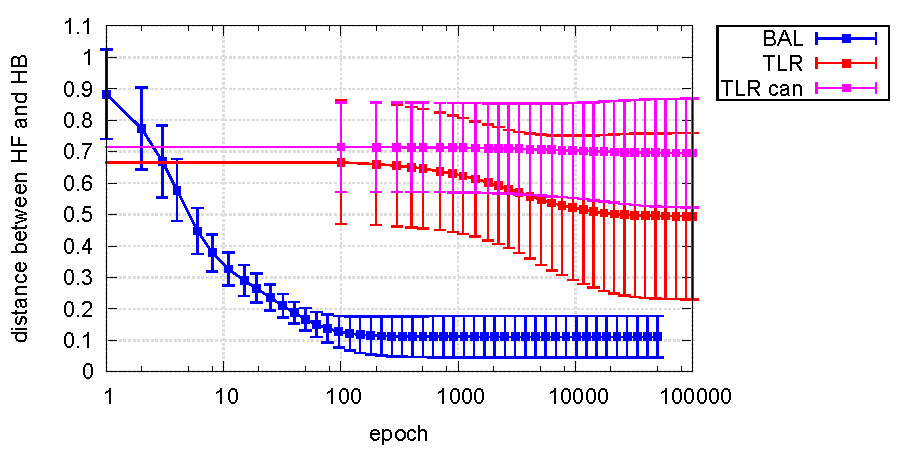
\includegraphics[width=0.6\textwidth]{img/feature-cmp-h-fb-d.pdf}  
   \caption{Comparing $dist_{H}^{FB}$~(\ref{sec:our-dist-h-fb}) evolution on the {4-2-4 encoder} task.}
  \label{fig:results-candidates-h-fb-d}
\end{figure}

\begin{figure}[H]
  \centering
  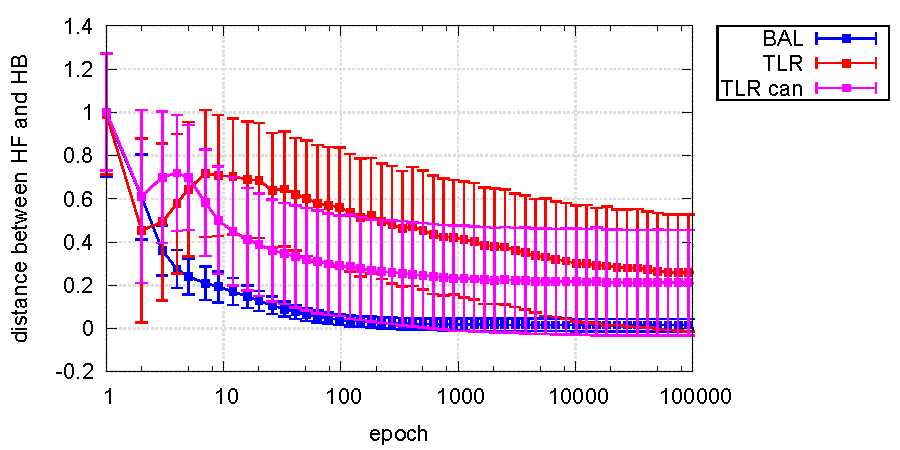
\includegraphics[width=0.6\textwidth]{img/feature-cmp-o-fb-d.pdf}  
   \caption{Comparing $dist_{O}^{FB}$~(\ref{sec:our-dist-o-fb}) evolution on the {4-2-4 encoder} task.}
  \label{fig:results-candidates-o-fb-d}
\end{figure}

\begin{figure}[H]
  \centering
  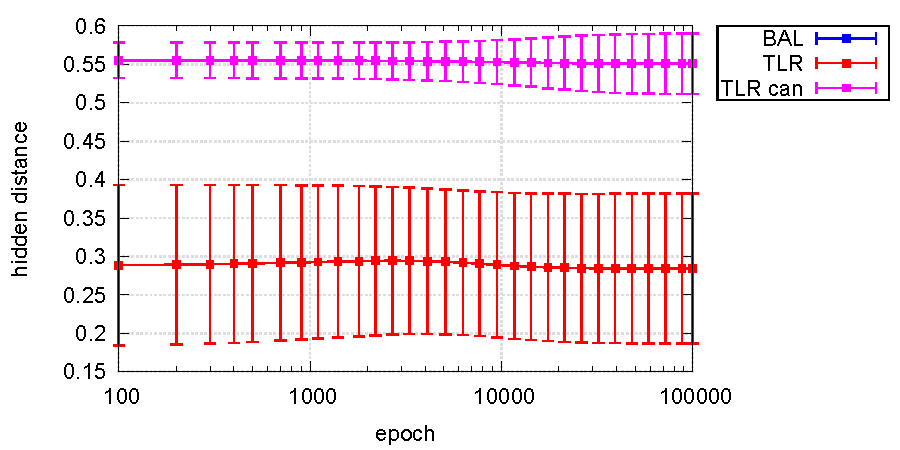
\includegraphics[width=0.6\textwidth]{img/feature-cmp-h-dist.pdf}  
   \caption{Comparing $dist_{H}$~(\ref{sec:our-h-dist}) evolution on the {4-2-4 encoder} task.}
  \label{fig:results-candidates-h-dist}
\end{figure}

\begin{figure}[H]
  \centering
  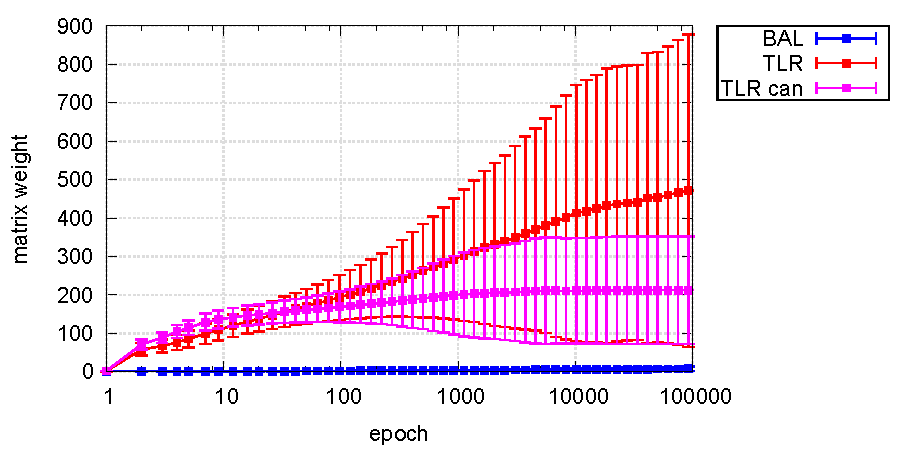
\includegraphics[width=0.6\textwidth]{img/feature-cmp-m-wei.pdf}  
   \caption{Comparing $matrix\_weight$~(\ref{sec:our-m-wei}) evolution on the {4-2-4 encoder} task.}
  \label{fig:results-candidates-m-wei}
\end{figure}


\subsubsection{Other}

\paragraph{Recirculation BAL.} 
In figure~\ref{fig:results-bal-recirc-auto4-performance} we see that \emph{BAL-recirc}~(\ref{sec:our-bal-recirc}) achieved lower success rate than BAL on the \emph{4-2-4 encoder} task. In comparison with TLR we see that there is a global maxima at point $\lambda_h = 0.0001$ and $\lambda_v=1.0$. We can therefore conclude that the space of successfull parameters $\lambda_h$ and $\lambda_v$ is bounded. Similar results were achieved for GeneRec as shown in figure~\ref{fig:results-generec-auto4-performance}.
%======== (3D) L1 x L2 x epochs =========
%======== (3D) L1 x L2 x patSuccF =========
\begin{figure}[H]
  \centering
  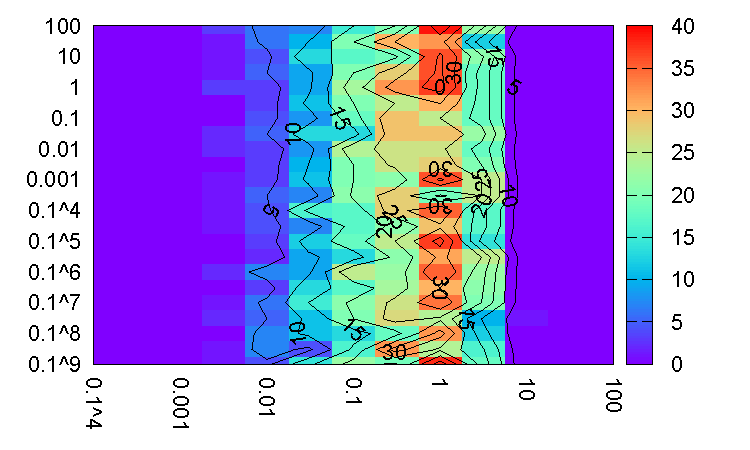
\includegraphics[width=0.49\textwidth]{img/bal-recirc-auto4-success.pdf}   
  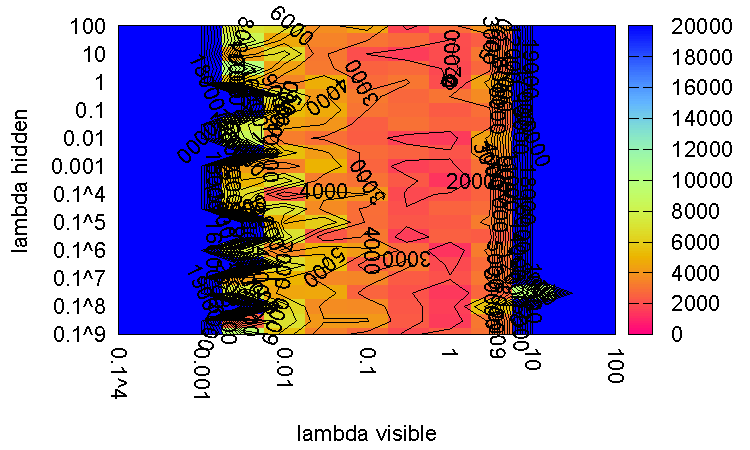
\includegraphics[width=0.49\textwidth]{img/bal-recirc-auto4-epoch.pdf}     
  \caption{BAL-recirc~(\ref{sec:our-bal-recirc}) success and epochs on the \emph{4-2-4 encoder}. Best result $36\%$ achieved with $\lambda_h = 0.0001$ and $\lambda_v=1.0$.}
  \label{fig:results-bal-recirc-auto4-performance}
\end{figure}
%success lambda_h lambda_v
%33.0 0.0003 1.0
%33.0 0.001 3.0
%34.0 0.01 1.0
%36.0 0.0001 1.0
%36.0 3.0e-05 0.3


\paragraph{GeneRec.} 
As with generalizing of BAL to TLR we tried also generalizing GeneRec using the two learning rates approach. The results in figure~\ref{fig:results-generec-auto4-performance} show no increase in success rate in comparison with setting $\lambda_v = \lambda_h$, i.e. using the original GeneRec. We can observe that the results are similar with the results of BAL-recirc shown in figure~\ref{fig:results-bal-recirc-auto4-performance}. Finally, as with BAL-recirc, we can conclude that the success space is bounded.  
%======== (3D) L1 x L2 x epochs =========the
%======== (3D) L1 x L2 x patSuccF =========
\begin{figure}[H]
  \centering
  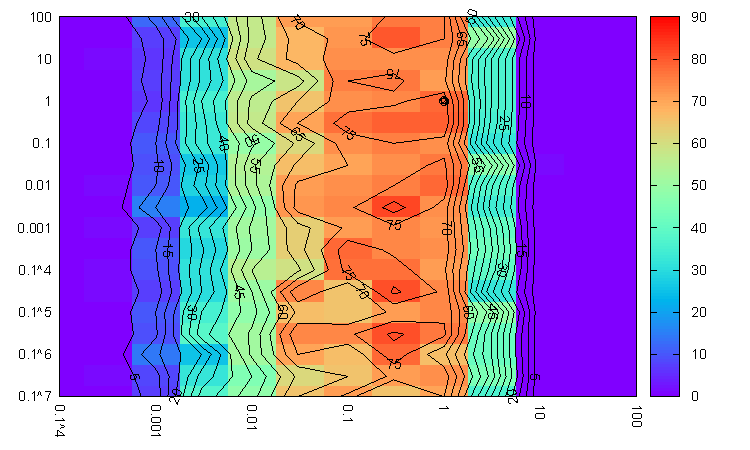
\includegraphics[width=0.49\textwidth]{img/generec-auto4-success.pdf}   
  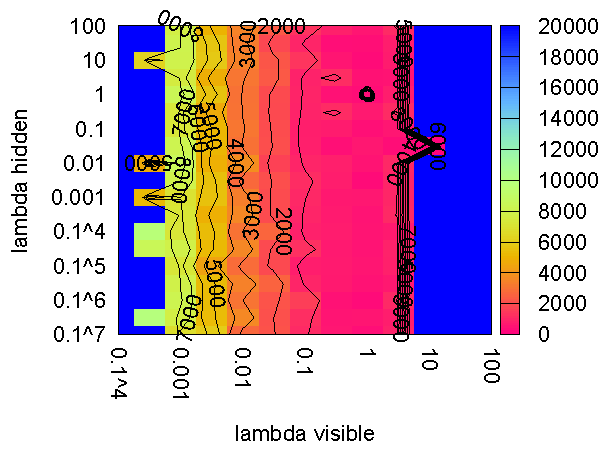
\includegraphics[width=0.49\textwidth]{img/generec-auto4-epoch.pdf}     
  \caption{GeneRec~(\ref{sec:models-generec}) success rate and convergence time on the \emph{4-2-4 encoder} task with $\sigma = 2.3$ and $\mu = 0.0$. Best result $83\%$ achieved with $\lambda_h = 0.3$ and $\lambda_v=1.0$.}
  \label{fig:results-generec-auto4-performance}
\end{figure}

%77.0 1.0 0.1
%78.0 1.0 0.3
%81.0 0.3 0.3
%83.0 0.3 1.0

%\paragraph{Symmetric BAL.} 
%\label{sec:our-bal-sym} 
%We were inspired by the necessary condition for convergence of GeneRec as stated by~\citet{o1996bio}. Thus we introduced \emph{Symmetric BAL (SymBAL)} as a modification of BAL where we set symmetric weights $W^{IH} = (W^{HI})^T$ and $W^{HO} = (W^{OH})^T$. We found no significant improvement when using this approach. 

\subsubsection{Conclusion} 
\label{sec:tlr-auto4-conclusion} 

\label{sec:tlr-auto4-hypothesis} 
The result in this chapter suggest a hypothesis why TLR outperforms BAL on the \emph{4-2-4 encoder task}. The reason is that the hidden activations settle before $W^{HO}$ and $W^{HI}$ adapt to them. This is explained by the fact that forward and backward hidden activations become same to fast~(\ref{sec:tlr-auto4-hidden},~\ref{sec:our-hidden-activation}) and the weight initialization could help this~(\ref{fig:results-tlr-auto4-epoch}). The first issue is solved by setting $\lambda_h \ll \lambda_h$ which adds epochs to the training phase. The second issue is solved by candidate selection which prevents initializing hidden activations close to each other. 

 

%Experimental Results and Analysis – in this section, you should show the quantitative results – charts and tables. Analyze the results by explaining and highlighting what is important on them in terms of your goals and what is bad. You should explain the strange results too.

%V ďalšej časti prezentujte vlastný prínos a vlastné výsledky porovnajte s výsledkami iných. Charakterizujte použité metódy.
%Vyhýbajte sa používaniu žargónu.
%Používajte starú múdrosť: 1 obrázok je viac než 1000 slov.

%============================================================
\subsection{Complex binary vector associations} 
\label{sec:results-k3}

In this section, we inspect TLR~(\ref{sec:our-tlr}) and GeneRec~(\ref{sec:models-generec}) performance on the \emph{CBVA} task~(\ref{sec:datasets-k3}). The methodology is similar as in case of the 4-2-4 encoder task described in \ref{sec:results-auto4-introduction}. The main difference is that we tried several architectures of type 16-$n$-16 for $n \in \{3,\,4,\cdots,\,10\}.$. Second difference was the setting of $Epoch_{\rm max}$ to 20,000 for TLR and 5,000 for GeneRec. 

%============================================================
\subsubsection{Two learning rates} 
\label{sec:tlr-k3}

On figure~(\ref{fig:results-tlr-k3-performance}) we compare success rate of TLR for different settings of $\lambda_v$ and $\lambda_h$ and different hidden sizes. We see that even for the 16-3-16 architecture TLR was able to learn the for ($\lambda_v, \lambda_h$) on the half line from  $(1, 0.1)$ to $(10^4, 0.1)$. This behaviour of TLR is similar to the behaviour of TLR on the \emph{4-2-4 encoder} task shown on figure~(\ref{fig:results-bal-recirc-auto4-performance}). Again, the performance mostly depends on $\lambda_h$ and it is bounded by a value of $\lambda_v$. Also, It is interesting how the success space expanded from top to down when increasing the hidden size.

%Main purpose of this dataset is to test different hidden sizes 
%======== (4D) L1 x L2 x patSuccF x hidden size =========
%======== (4D) L1 x L2 x epochs x hidden size =========

\begin{figure}[H]
  \centering
  %Hidden size = 3 \\
  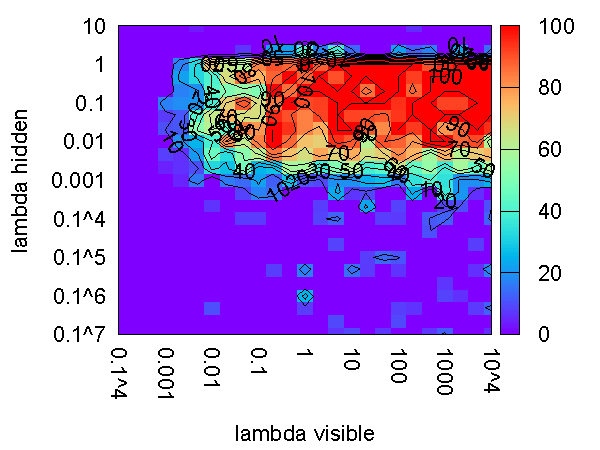
\includegraphics[width=0.49\textwidth]{img/k3/tlr-3-success.pdf} 
  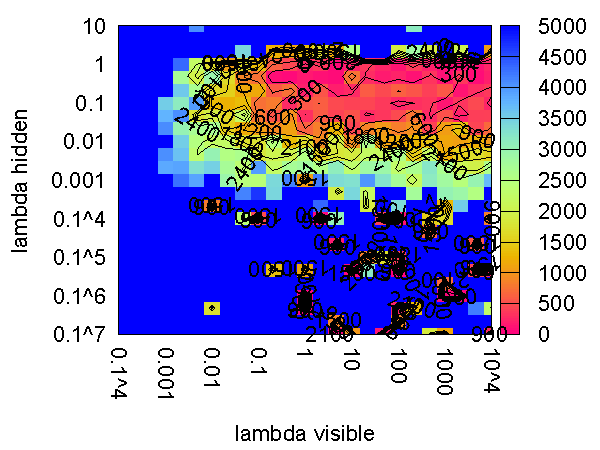
\includegraphics[width=0.49\textwidth]{img/k3/tlr-3-epoch.pdf}   
  %Hidden size = 4 \\
  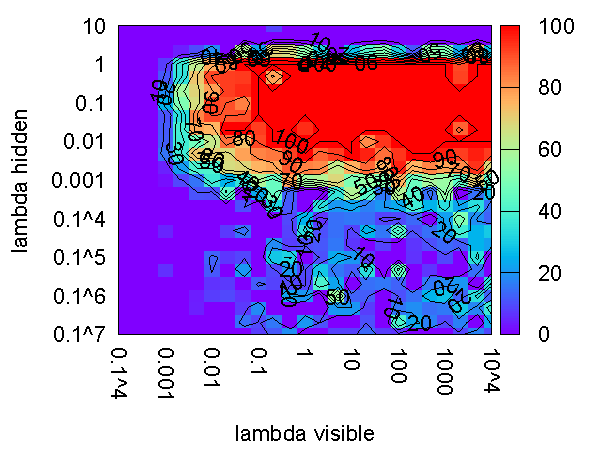
\includegraphics[width=0.49\textwidth]{img/k3/tlr-4-success.pdf} 
  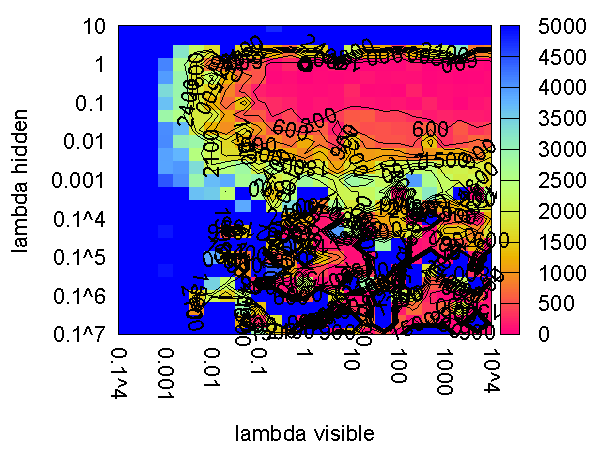
\includegraphics[width=0.49\textwidth]{img/k3/tlr-4-epoch.pdf}   
  %Hidden size = 5 \\
  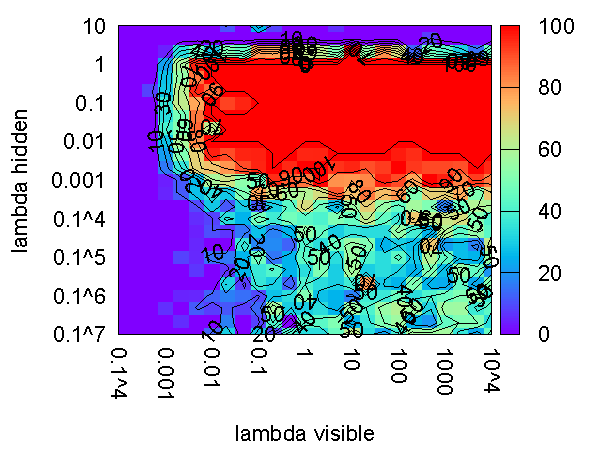
\includegraphics[width=0.49\textwidth]{img/k3/tlr-5-success.pdf}   
  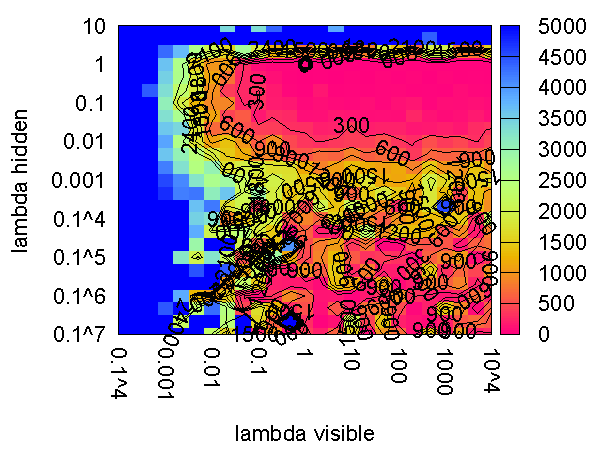
\includegraphics[width=0.49\textwidth]{img/k3/tlr-5-epoch.pdf}  
  %Hidden size = 8 \\
  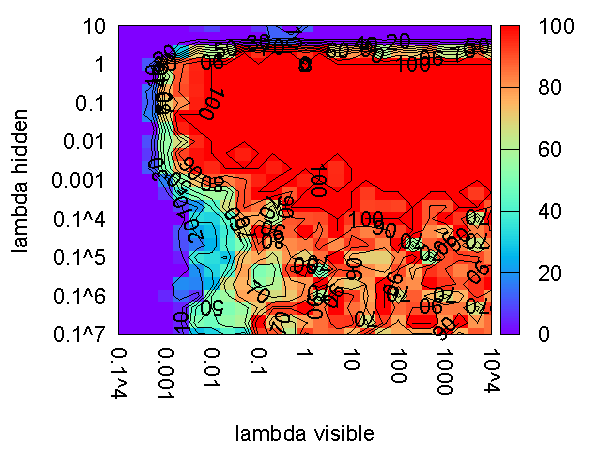
\includegraphics[width=0.49\textwidth]{img/k3/tlr-7-success.pdf} 
  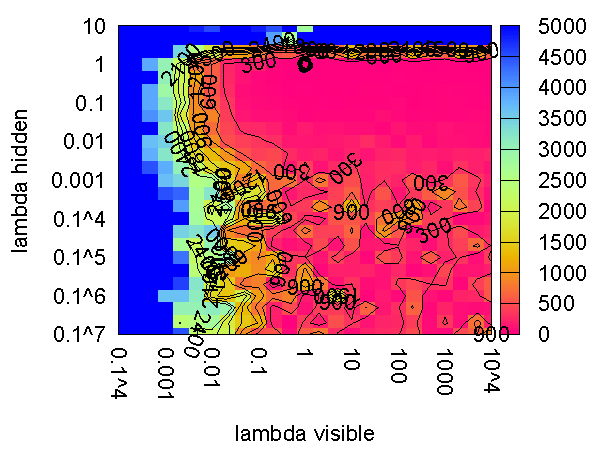
\includegraphics[width=0.49\textwidth]{img/k3/tlr-7-epoch.pdf}    
  \caption{TLR performance on the \emph{CBVA} task with hidden sizes 3, 4, 5 and 7 from top to bottom.}
  \label{fig:results-tlr-k3-performance}
\end{figure}

On figure~\ref{fig:results-tlr-auto4-epoch} the success timeline for TLR with best $\lambda_h$ and $\lambda_v$ is inspected. We can observe that TLR is increasing its success in time steadily. Moreover, we see that the candidate preselection~(\ref{sec:sim-exp-candidates}) has an positive impact on the network performance.
Note that as the CBVA task is non bijective, i.e. one output has several inputs, it is impossible to achieve 100\% $patSucc^B$ or $bitSucc^B$. 

%======== (3D) best TLR on ALL_SUCC x epoch (std-dev) x hidden size ==========
\begin{figure}[H]
  \centering
  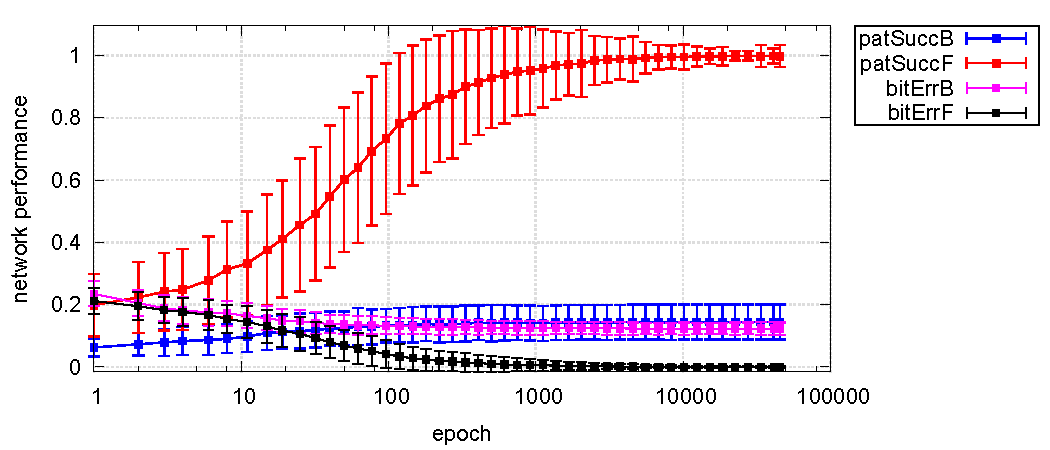
\includegraphics[width=0.8\textwidth]{img/tlr-k3-3-best-perf.pdf}   
  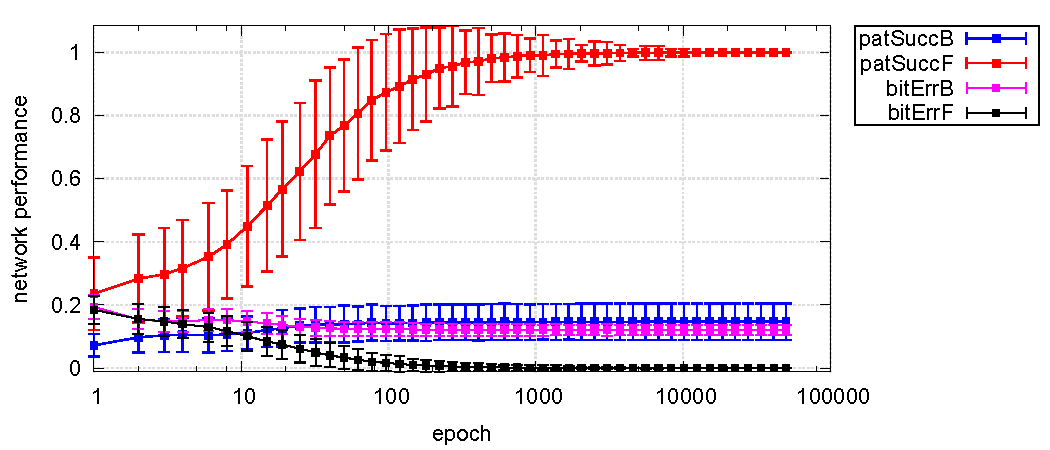
\includegraphics[width=0.8\textwidth]{img/tlr-k3-3-best-can.pdf}      
  \caption{TLR success timeline for the \emph{CBVA} task with $\lambda_h=0.1$ and $\lambda_v=100$. Top without candidate selection and bottom with candidate selection. }
  \label{fig:results-tlr-k3-epoch} 
\end{figure}

\subsubsection{Comparison} 
\label{sec:results-cmp-k3} 

In table~(\ref{tab:results-cmp-k3}) the comparison of TLR and Generec on the \emph{CBVA} task is shown. TODO rerun bugfix and explain 

%===== TODO table: best parameter setting networks with hidden.size= constant (success, epoch, stddev) / model \\

\begin{table}[H] 
  \centering
    \begin{tabular}{|l|l|l|l|l|}
    \hline
    Algorithm (section)&$\lambda_h$&$\lambda_v$&$patSucc^F$ &Epochs\\ %&SEM(success) \\
    \hline
    GR~(\ref{sec:models-generec}) & & & & \\ %&28\\
    \hline
    GR TLR & & & & \\ %&28\\
    \hline
    BAL~(\ref{sec:models-bal})&0.5& 0.5&100& 54\\ %&2.0e+08\\
    \hline
    BAL TLR~(\ref{sec:our-tlr})&1.0& 5.0 & 100& 64\\ %&1.52e+08\\
    %\hline
    %BAL TLR Can~(\ref{sec:sim-exp-candidates})& & & & \\ %&5,070,000\\ 
    \hline 
    \end{tabular}
  \caption{Comparing performance of different models on the \emph{4-2-4 encoder} task with 3 hidden neurons. } 
  \label{tab:results-cmp-k3}
\end{table}

%SELECT lambda, lambda_ih, 100*AVG(success) AS 'suc', AVG(epoch) AS 'epc' FROM data WHERE epoch <> 0 GROUP BY lambda,lambda_ih ORDER BY suc ASC, epc DESC; 
%generec tlr

%generec pure 

%tlr pure 
%2.0|0.5|100.0|98.7777777777778
%2000.0|1.0|100.0|86.48
%5000.0|0.5|100.0|77.1428571428571
%5.0|1.0|100.0|64.0
%0.5|0.5|100.0|54.0

%tlr candidate 


\subsubsection{GeneRec} 

On figure~\ref{fig:results-tlr-k3-performance} we compare success rate of TLR for different settings of $\lambda_v$ and $\lambda_h$ and different hidden sizes. TODO rerun bugfix and explain 

\begin{figure}[H]
  \centering
  Hidden size = 3 \\
  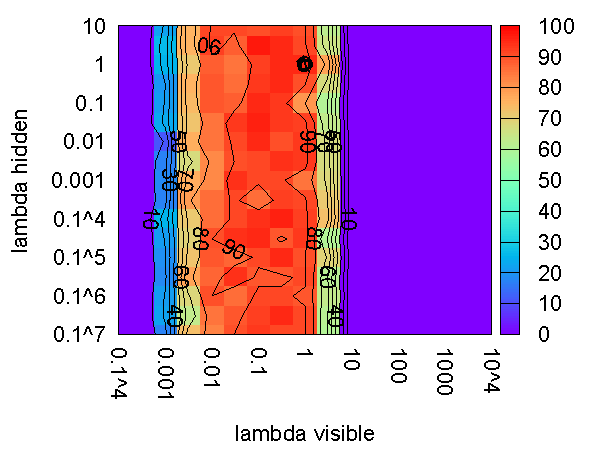
\includegraphics[width=0.49\textwidth]{img/k3/generec-3-success.pdf} 
  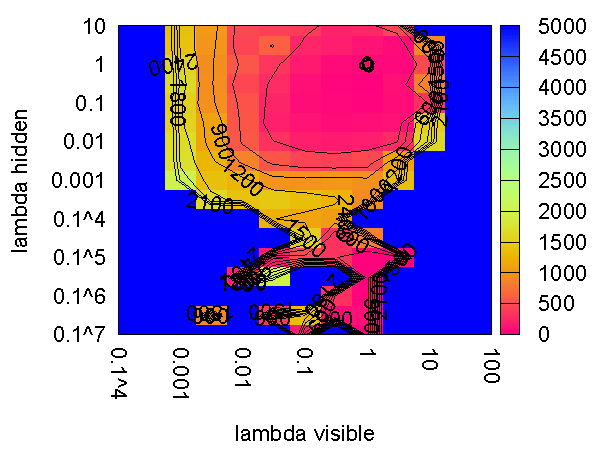
\includegraphics[width=0.49\textwidth]{img/k3/generec-3-epoch.pdf}   
%  Hidden size = 4 \\
%  \includegraphics[width=0.49\textwidth]{img/k3/generec-4-success.pdf} 
%  \includegraphics[width=0.49\textwidth]{img/k3/generec-4-epoch.pdf}   
  Hidden size = 5 \\
  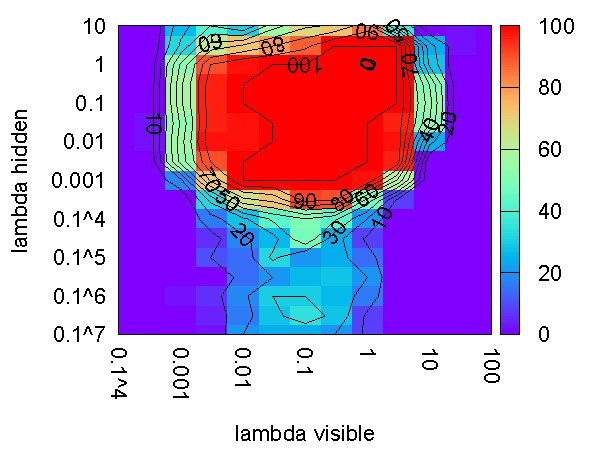
\includegraphics[width=0.49\textwidth]{img/k3/generec-5-success.pdf} 
  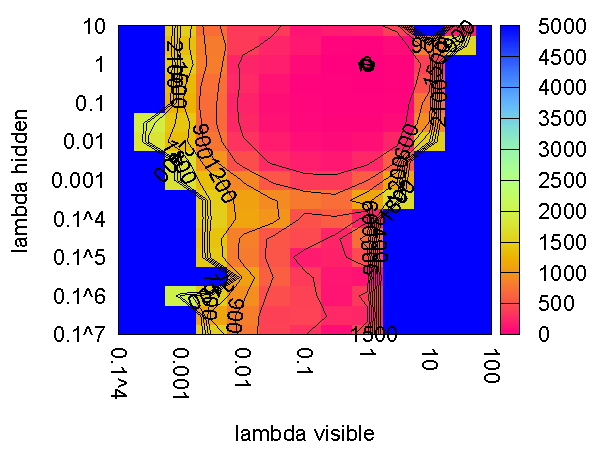
\includegraphics[width=0.49\textwidth]{img/k3/generec-5-epoch.pdf}  
%  Hidden size = 7 \\
%  \includegraphics[width=0.49\textwidth]{img/k3/generec-7-success.pdf} 
%  \includegraphics[width=0.49\textwidth]{img/k3/generec-7-epoch.pdf}    
  \caption{\emph{GeneRec} performance on the \emph{CBVA} task with different hidden sizes.} %For greater hidden sizes the results were very similar to the results with hidden size 5.}
  \label{fig:results-generec-k3-success}
\end{figure}

 

%Experimental Results and Analysis – in this section, you should show the quantitative results – charts and tables. Analyze the results by explaining and highlighting what is important on them in terms of your goals and what is bad. You should explain the strange results too.

%V ďalšej časti prezentujte vlastný prínos a vlastné výsledky porovnajte s výsledkami iných. Charakterizujte použité metódy.
%Vyhýbajte sa používaniu žargónu.
%Používajte starú múdrosť: 1 obrázok je viac než 1000 slov.

\subsection{Handwritten Digits} 
\label{sec:results-digits} 

(\ref{sec:datasets-digits}) 

%===============================================================
%===============================================================
%===============================================================
\subsubsection{Two learning rates} 
\label{sec:tlr-digits} 

%Purpose: 
%======== (3D) L1 x L2 x patSuccF =========
%======== (3D) L1 x L2 x epochs =========
\begin{figure}[H]
  \centering
  \includegraphics[width=0.60\textwidth]{img/tlr-digits-psf.pdf} 
%  \includegraphics[width=0.49\textwidth]{img/tlr-digits-epoch.pdf}     
  \caption{TLR performance on the \emph{digits} task for $\mu = 0.01$.}
  \label{fig:results-tlr-digits-success}
\end{figure}

%======== (2D) best TLR on ALL_SUCC x epoch (std-dev) ==========
\begin{figure}[H]
  \centering
  \includegraphics[width=0.45\textwidth]{img/placeholder.png}  %TODO    
  \caption{TLR success evolution for the \emph{digits} task.}
  \label{fig:results-tlr-digits-epoch} 
\end{figure}

%===============================================================
%===============================================================
%===============================================================
\subsubsection{Comparison} 
\label{sec:results-cmp-digits} 
TODO simulation + plots~(\ref{sec:datasets-digits}) 

For TLR, BAL, GeneRec + known performers 
TODO: table: best parameter setting networks with hidden.size= constant (success, epoch, stddev) / model \\

\begin{table}[H] 
  \centering
    \begin{tabular}{|l|l|l|l|l|}
    \hline
    Algorithm (section)&$\lambda_h$&$\lambda_v$&$patSucc^F$ &Epochs\\ %&SEM(success) \\
    \hline
    BAL TLR~(\ref{sec:our-tlr})& & & & \\ %&1.52e+08\\
    \hline 
    \end{tabular}
  \caption{Comparing performance of different models on the \emph{digits} task with 300 hidden neurons.} 
  \label{tab:results-cmp-digits}
\end{table}

\paragraph{Backward representations.} 
(\ref{sec:our-backward-repre}) 

TODO 3x 10x backward digit representations 

\begin{figure}[H]
  \centering
  \includegraphics{../presentation/img/dig_0.png} %TODO 
  \includegraphics{../presentation/img/dig_1.png} 
  \includegraphics{../presentation/img/dig_2.png} 
  \includegraphics{../presentation/img/dig_3.png} 
  \includegraphics{../presentation/img/dig_4.png} 
  \includegraphics{../presentation/img/dig_5.png} 
  \includegraphics{../presentation/img/dig_6.png} 
  \includegraphics{../presentation/img/dig_7.png} 
  \includegraphics{../presentation/img/dig_8.png} 
  \includegraphics{../presentation/img/dig_9.png} 
  \caption{Backward representations on \emph{digits} for GeneRec.}
  \label{fig:results-backward-repre-generec}
\end{figure}


%===============================================================
%===============================================================
%===============================================================
\subsubsection{Backward representations} 

\label{sec:our-backward-repre}

The method of \emph{backward representations} for \emph{hetero--associative} tasks, i.e.~tasks which have multiple inputs for the same output, is to \emph{depict} the backward activation of all possible outputs. In case of BAL~(\ref{sec:models-bal}) the backward representations are all possible values of $x^{\rm B}$. For example the backward representation of digit "8" in TLR~(\ref{sec:our-tlr}) is show on figure~\ref{fig:our-backward-repre}. 

\begin{figure}[H]
  \centering
  \includegraphics[width=0.2\textwidth]{img/tlr-digit-8.png} %TODO 
  \caption{Backward representation of digit "8" in TLR.}
  \label{fig:our-backward-repre}
\end{figure}

%======== (2D) for best network vs. sample digits
\begin{figure}[H]
%TODO rotate 
  \centering
  \includegraphics[width=0.45\textwidth]{img/tlr-digits.png}    
  \caption{Best TLR backward representations for the \emph{digits} task.}
  \label{fig:results-tlr-digits-backward} 
\end{figure}
 


\subsubsection{Important features}
\label{sec:results-candidates} 

With the candidate selection experiment \ref{sec:sim-exp-candidates} we have found the most important features. 

TODO Hidden distance (over 70\%); in triangle (68.3 \%). \\

%======== (3D) L1 x L2 x patSuccF : TLR vs. CS-TLR =========
%======== (3D) L1 x L2 x epochs : TLR vs. CS-TLR =========

\begin{figure}[H]
  \centering
  \includegraphics[width=0.45\textwidth]{img/placeholder.png}  %TODO   
  \includegraphics[width=0.45\textwidth]{img/placeholder.png}  %TODO    
  \caption{Candidate selection. Selecting highest \emph{hidden distance} among 1000 randomly generated networks leads to $\approx 10\%$ success increase.}
  \label{fig:results-candidates-tlr}
\end{figure}

%======== (2D) best TLR on ALL_SUCC x epoch (std-dev) : TLR vs. CS-TLR ==========

\begin{figure}[H]
  \centering
  \includegraphics[width=0.45\textwidth]{img/placeholder.png}  %TODO   
  \includegraphics[width=0.45\textwidth]{img/placeholder.png}  %TODO    
  \caption{Comparing candidate selection to standard BAL.}
  \label{fig:results-candidates-epoch}
\end{figure}

\paragraph{Linear regression model.} 

Following our best feature selection process \ref{sec:sim-exp-candidates} we trained a linear regression model over the network measures with label being $1-\mbox{bitSucc}^F = \mbox{bitErr}^F$. TODO explain more 
\begin{align} 
\label{eq:results-candidates-linear-regression} 
\mbox{bitErr}^F &= 
- 0.328 \times \mbox{dist}_{H}
+ 0.140 \times \mbox{dist}_{H}^{FB}
- 0.100 \times \mbox{dist}_{O}^{FB} \nonumber \\
&+ 0.019 \times matrix\_sim
- 0.127 \times \sigma
+ 3.610
\end{align} 

\paragraph{Comparing feature evolution of TLR to BAL.} 

TODO add plots of feature / epoch for the best TLR and BAL. 

\begin{figure}[H]
  \centering
  \includegraphics[width=0.45\textwidth]{img/placeholder.png}  %TODO   
  \includegraphics[width=0.45\textwidth]{img/placeholder.png}  %TODO    
  \caption{Evolution of the distance between forward and backward hidden activations $\mbox{dist}_{H}^{FB}$ \ref{sec:our-dist-h-fb}. Further discussion in \ref{sec:our-hidden-activation}. }
  \label{fig:results-candidates-dist-h-fb}
\end{figure}

 


\subsection{Observations}
\label{sec:results-tlr}  %TODO (still relevant label? ) 

Other partial results we found interesting. 
TODO talk about these points (item -> paragraph ; item -> other results): 


\subsubsection{Important features}
\label{sec:results-candidates} 

With the candidate selection experiment \ref{sec:sim-exp-candidates} we have found the most important features. 

TODO Hidden distance (over 70\%); in triangle (68.3 \%). \\

%======== (3D) L1 x L2 x patSuccF : TLR vs. CS-TLR =========
%======== (3D) L1 x L2 x epochs : TLR vs. CS-TLR =========

\begin{figure}[H]
  \centering
  \includegraphics[width=0.45\textwidth]{img/placeholder.png}  %TODO   
  \includegraphics[width=0.45\textwidth]{img/placeholder.png}  %TODO    
  \caption{Candidate selection. Selecting highest \emph{hidden distance} among 1000 randomly generated networks leads to $\approx 10\%$ success increase.}
  \label{fig:results-candidates-tlr}
\end{figure}

%======== (2D) best TLR on ALL_SUCC x epoch (std-dev) : TLR vs. CS-TLR ==========

\begin{figure}[H]
  \centering
  \includegraphics[width=0.45\textwidth]{img/placeholder.png}  %TODO   
  \includegraphics[width=0.45\textwidth]{img/placeholder.png}  %TODO    
  \caption{Comparing candidate selection to standard BAL.}
  \label{fig:results-candidates-epoch}
\end{figure}

\paragraph{Linear regression model.} 

Following our best feature selection process \ref{sec:sim-exp-candidates} we trained a linear regression model over the network measures with label being $1-\mbox{bitSucc}^F = \mbox{bitErr}^F$. TODO explain more 
\begin{align} 
\label{eq:results-candidates-linear-regression} 
\mbox{bitErr}^F &= 
- 0.328 \times \mbox{dist}_{H}
+ 0.140 \times \mbox{dist}_{H}^{FB}
- 0.100 \times \mbox{dist}_{O}^{FB} \nonumber \\
&+ 0.019 \times matrix\_sim
- 0.127 \times \sigma
+ 3.610
\end{align} 

\paragraph{Comparing feature evolution of TLR to BAL.} 

TODO add plots of feature / epoch for the best TLR and BAL. 

\begin{figure}[H]
  \centering
  \includegraphics[width=0.45\textwidth]{img/placeholder.png}  %TODO   
  \includegraphics[width=0.45\textwidth]{img/placeholder.png}  %TODO    
  \caption{Evolution of the distance between forward and backward hidden activations $\mbox{dist}_{H}^{FB}$ \ref{sec:our-dist-h-fb}. Further discussion in \ref{sec:our-hidden-activation}. }
  \label{fig:results-candidates-dist-h-fb}
\end{figure}

 

\subsubsection{Momentum}
\label{sec:results-momentum} 

\ref{sec:our-momentum} 
%======== (3D) L1 x L2 x patSuccF : TLR vs. best momentum =========
%======== (3D) L1 x L2 x epochs : TLR vs. best momentum =========

\begin{figure}[H]
  \centering
  \includegraphics[width=0.45\textwidth]{img/placeholder.png}  %TODO
  \includegraphics[width=0.45\textwidth]{img/placeholder.png}  %TODO
  \caption{Comparing different \emph{momentums} for TLR on the \emph{4-2-4 encoder} task.}
  \label{fig:results-tlr-auto4-momentum}
\end{figure}

%======== (2D) best TLR on ALL_SUCC x epoch (std-dev) : TLR vs. best momentum ==========

\subsubsection{Weight initialization}
\label{sec:results-sigma} 

\ref{sec:our-sigma} 

\begin{figure}[H]
  \centering
  \includegraphics[width=0.45\textwidth]{img/placeholder.png}  %TODO   
  \includegraphics[width=0.45\textwidth]{img/placeholder.png}  %TODO    
  \caption{Comparing different \emph{weight initializations} for TLR on the \emph{4-2-4 encoder} task.}
  \label{fig:results-tlr-auto4-sigma}
\end{figure}
%======== (3D) L1 x L2 x patSuccF : TLR vs. best sigma =========
%======== (3D) L1 x L2 x epochs : TLR vs. best sigma =========
%======== (2D) best TLR on ALL_SUCC x epoch (std-dev) : TLR vs. best sigma ==========

\subsubsection{Long run} 
\label{sec:results-long-run} 

%======== (3D) L1 x L2 x patSuccF : TLR vs. long run best =========
%======== (3D) L1 x L2 x epochs : TLR vs. long run best =========
\begin{figure}[H]
  \centering
  \includegraphics[width=0.45\textwidth]{img/placeholder.png}  %TODO   
  \includegraphics[width=0.45\textwidth]{img/placeholder.png}  %TODO    
  \caption{Running 1,000,000 epochs on the \emph{4-2-4 encoder} task with BAL. This could lead to $\approx 10\%$ success increase.}
  \label{fig:results-tlr-auto4-long-run}
\end{figure}


%======== (2D) best TLR on ALL_SUCC x epoch (std-dev) : TLR vs. long run best ==========


\subsubsection{Other}

\begin{itemize} 
\item Matrices IH-OH and HO-HI tend to be same in autoassociative tasks. 
\item Hidden representation distance is a meaningful measure (LinReg on pre\_measure) (+ 10\%) . 
\item In triangle (non-convex). Not-in triangle is a must to condition for success. \\
TODO rerun to get "1 err in\_triangle" with and without preselection (there was a bug in the old data). 
\item reprezentacie na hidden absolutne rovnake (forward, backward), matice rozne:
\item Convergence Epsilon - weights tend to infinity (09-12-2013: Convergence which depends on average weight change does not work). 
\item Rerun - same config, different order when training 
All bad: \\
err sigma lambda momentum success sample\_ratio \\
0.0 2.3 0.7 0.0 19.296918767507005 6889/35700 \\
1.0 2.3 0.7 0.0 68.05602240896359 24296/35700 \\
2.0 2.3 0.7 0.0 12.644257703081232 4514/35700 \\
3.0 2.3 0.7 0.0 0.0028011204481792717 1/35700 \\

All good:  \\
err sigma lambda momentum success sample\_ratio \\
0.0 2.3 0.7 0.0 99.98911353032659 64293/64300 \\
1.0 2.3 0.7 0.0 0.01088646967340591 7/64300 \\
\end{itemize}
 
 




 

%V ďalšej časti prezentujte vlastný prínos a vlastné výsledky porovnajte s výsledkami iných. Charakterizujte použité metódy.
%Vyhýbajte sa používaniu žargónu.
%Používajte starú múdrosť: 1 obrázok je viac než 1000 slov.

\subsection{Comparison} 
\label{sec:results-comparison}

TODO: GNUPlot std bars \\  
TODO: Introduce shortcuts and add references to descriptions. \\

\subsubsection{4-2-4 Encoder}

For all our models \ref{sec:our-models} tested on the 4-2-4 encoder task~\ref{sec:datasets-auto4} the two learning rate model~\ref{sec:our-two-lambdas} had the best success rate. 

For TLR, BAL, GeneRec, BP, CHL, other learning rules
TODO: success / epochs  \\
TODO: table: best parameter setting networks (success, epoch, stddev) / model \\

\paragraph{Hidden activations.} 

TODO hidden activation timelines with commentaries (for TLR, BAL, GeneRec) 
2x success, 2x error (wrong settle, divergence) 

\subsubsection{Complex Binary Vector Associations}
\ref{sec:datasets-k3} 

For TLR, BAL, GeneRec, other learning rules
TODO: bitSucc, patSucc / epochs  \\
TODO: success / hidden layer size  \\
TODO: table: best parameter setting networks with hidden.size= constant (success, epoch, stddev) / model \\

\subsubsection{Hand--written digits.}
TODO simulation + plots \ref{sec:datasets-digits} 

For TLR, BAL, GeneRec + known performers 
TODO: table: best parameter setting networks with hidden.size= constant (success, epoch, stddev) / model \\

\paragraph{Backward representations.} 

TODO 3x 10x backward digit representations 
 

